\documentclass[12pt, letterpaper, twoside]{article}

\usepackage{geometry}
\usepackage{graphicx}
\usepackage{amsmath, amsfonts, amssymb, bbm}
%\usepackage{lipsum}
\usepackage{fancyhdr}
%\usepackage{layout}
\usepackage{lettrine}
\usepackage[explicit]{titlesec}
\usepackage{hyperref}
\usepackage{watermark}
\usepackage{color}


%%%%%%%%%%%%%%%%%%%%%%%% 
% FONT SELECTION  
%%%%%%%%%%%%%%%%%%%%%%%% 

\usepackage[light]{iwona}
\usepackage[T1]{fontenc}

%%%%%%%%%%%%%%%%%%%%%%%%
% DEFINE COLORS
%%%%%%%%%%%%%%%%%%%%%%%%

\definecolor{grey}{rgb}{0.5,0.5,0.5}
\definecolor{l-grey}{rgb}{0.8,0.8,0.8}
\definecolor{withe}{rgb}{1,1,1}
\definecolor{black}{rgb}{0,0,0}

%%%%%%%%%%%%%%%%%%%%%%%% 
% PAGE LAYOUT
%%%%%%%%%%%%%%%%%%%%%%%%

% Paper Width 614pt
% Text fill symemetric 604pt
% Paper Height 794pt

\setlength{\voffset}{-0.5in}
\setlength{\hoffset}{-1in}
\setlength{\oddsidemargin}{65pt}
\setlength{\evensidemargin}{45pt}
\setlength{\topmargin}{0in}
\setlength{\headheight}{15pt}
\setlength{\headsep}{20pt}
\setlength{\marginparwidth}{0in}
\setlength{\marginparsep}{0in}
\setlength{\textheight}{635pt}
\setlength{\textwidth}{494pt}
\setlength{\footskip}{50pt}

%%%%%%%%%%%%%%%%%%%%%%%%
% TITLES LAYOUT
%%%%%%%%%%%%%%%%%%%%%%%%

\titleformat{\section}[display]
{\vspace*{150pt}
\bf\Huge}
{\begin{picture}(0,0)\put(-60,-30){\textcolor{grey}{\thesection}}\end{picture}}
{0pt}
{#1}
[]
\titlespacing*{\section}{40pt}{10pt}{40pt}[40pt]
\newcommand{\sectionbreak}{\cleardoublepage}


%%%%%%%%%%%%%%%%%%%%%%%%
% MATH OPERATORS AND 
% CUSTOM ENVIRONMENTS
%%%%%%%%%%%%%%%%%%%%%%%%
\DeclareMathOperator{\Tr}{Tr}
\DeclareMathOperator*{\Cov}{Cov}
\DeclareMathOperator{\cov}{Cov} 
  
\newcounter{observ}
\newenvironment{observ}{\refstepcounter{observ}
   \textit{\textbf{Observation \theobserv:}} \rmfamily}
     
\newenvironment{proof}{\textit{Proof:} \rmfamily}{\hfill$\square$}

\newcommand{\ket}[1]{\ensuremath{\vert #1 \rangle}}
\newcommand{\bra}[1]{\ensuremath{\langle #1 \vert}} 
\newcommand{\braket}[2]{\ensuremath{\langle #1 \vert #2 \rangle}} 
\newcommand{\braOket}[3]{\ensuremath{\langle #1 \vert #2 \vert #3 \rangle}}
\newcommand{\ketbra}[2]{\ensuremath{\vert #1 \rangle \! \langle #2 \vert}}
\newcommand{\meanO}[1]{\ensuremath{\langle #1 \rangle}}
\newcommand{\ver}[2]{\ensuremath{\genfrac{}{}{0pt}{}{#1}{#2}}}
\newcommand{\tr}[1]{\ensuremath{\Tr \lcua #1\rcua}}
\newcommand{\trsub}[2]{\ensuremath{\Tr_{#1} \lcua #2 \rcua }}
\newcommand{\bsym}[1]{\ensuremath{\boldsymbol{#1}}}

\def\be{\begin{equation}}
\def\ee{\end{equation}}
\def\bea{\begin{eqnarray}}
\def\eea{\end{eqnarray}}
\def\bse{\begin{subequations}} 
\def\ese{\end{subequations}}
\def\mtxid{\mathbbm{1}}
\def\lpar{\left(} 
\def\rpar{\right)}
\def\lcua{\left[}
\def\rcua{\right]}
\def\lcor{\left\{}
\def\rcor{\right\}}
\def\lang{\left\langle}
\def\rang{\right\rangle}
\def\l{\left} 
\def\r{\right}
\def\nnnl{\nonumber\\}
\def\nnnlq{\nonumber\\ && \quad}
\def\nnnlqq{\nonumber\\ && \qquad}
\def\nnnlqqq{\nonumber\\ && \quad\qquad}
\def\ie{, \textit{i.e.}, }

%%%%%%%%%%%%%%%%%%%%%%%%
% DOCUMENT
%%%%%%%%%%%%%%%%%%%%%%%%

\begin{document}


\pagestyle{fancy}
\renewcommand{\headrulewidth}{0pt}
\fancyhead{}
\fancyfoot{}

%%%%%%%%%%%%%%%%%%%%%%%%
% TITLE PAGE 
%%%%%%%%%%%%%%%%%%%%%%%%

%!TEX root = main.tex 

\thiswatermark{\centering
\put(0,-110){
\includegraphics[height=2.5cm]{img/0-Ztf.png}} 
\put(430,-100){
\includegraphics[height=2cm]{img/0-Ehu.png}}
} 

\begin{center}

\vspace*{20pt}
\textsc{\LARGE University of the Basque Country}

\vspace{20pt}
\textsc{\Large PhD Thesis}

\vspace{50pt} 
\hrule 

\vspace{16pt}
{\huge \bfseries Lower bounds on quantum metrological precisions}
\vspace{16pt}

\hrule
\vspace{40pt}

\begin{minipage}{0.4\textwidth}
\begin{flushleft} \large
\emph{Author:}


M. Sc. Iagoba \textsc{Apellaniz}
\end{flushleft}
\end{minipage}
\begin{minipage}{0.4\textwidth}
\begin{flushright} \large
\emph{Director:}

Prof. G\'eza \textsc{T\'oth} %TODO: Check Geza's name
\end{flushright}
\end{minipage}

\vspace{40pt}
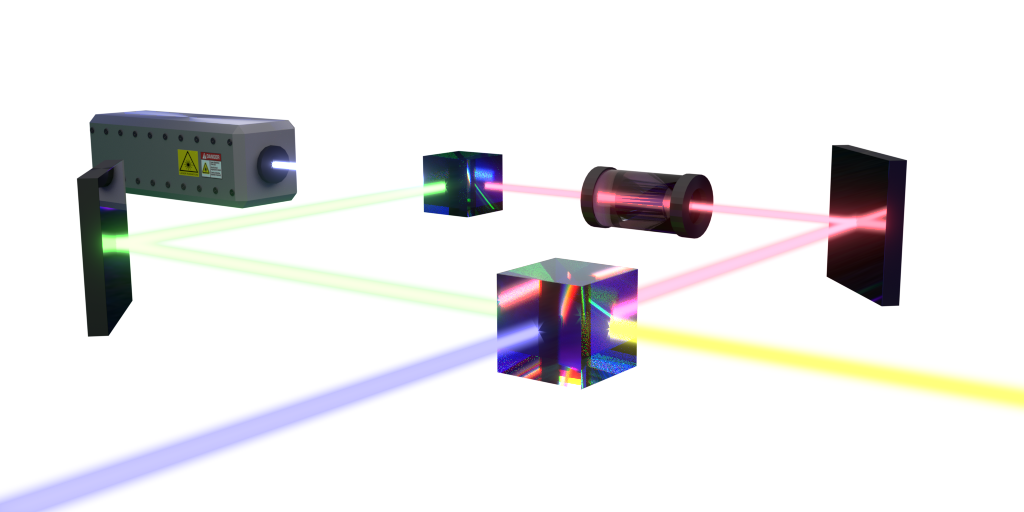
\includegraphics[width=0.8\hsize]{img/cover3Dpicture.png}
\vfill

% Bottom of the page
{\large \today}

\end{center}

\cleardoublepage

%%%%%%%%%%%%%%%%%%%%%%%%
% EDITION TIPS
%%%%%%%%%%%%%%%%%%%%%%%%

\cleardoublepage

This document was generated with the 2014 distribution of \LaTeX. 

\vfill


\includegraphics[height=20pt]{img/0-CreativeCommons-by-sa.png}

2012-2015 Iagoba Apellaniz. This work is licensed under the Creative Commons
Attribution-ShareAlike 4.0 International License. To view a copy of this
license, visit
\href{http://creativecommons.org/licenses/by-sa/4.0/deed.en_US}
{http://creativecommons.org/ licenses/by-sa/4.0/deed.en\_US}.
\clearpage

%%%%%%%%%%%%%%%%%%%%%%%%
% PROLOGE
%%%%%%%%%%%%%%%%%%%%%%%%

\section*{Prologue}
\setcounter{page}{1}
\pagenumbering{roman}
\fancyfoot[LE,RO]{\thepage}

Here is the prologue.

%%%%%%%%%%%%%%%%%%%%%%%%
% TABLE OF CONTENTS
%%%%%%%%%%%%%%%%%%%%%%%%

\vspace*{100pt}
\tableofcontents

\section*{Tables, figures and abbreviations used in this book}
\fancyfoot[LE,RO]{\thepage}

[Insert in a table]

SLD - Symmetric logarithmic derivative.

qFI - Quantum Fisher information

%%%%%%%%%%%%%%%%%%%%%%%%
% THESIS
%%%%%%%%%%%%%%%%%%%%%%%%

\cleardoublepage

\pagenumbering{arabic}
\fancyfoot{}
%!TEX root = main.tex 

\thiswatermark{\centering
\put(0,-110){
\includegraphics[height=2.5cm]{img/0-Ztf.png}} 
\put(430,-100){
\includegraphics[height=2cm]{img/0-Ehu.png}}
} 

\begin{center}

\vspace*{20pt}
\textsc{\LARGE University of the Basque Country}

\vspace{20pt}
\textsc{\Large PhD Thesis}

\vspace{50pt} 
\hrule 

\vspace{16pt}
{\huge \bfseries Lower bounds on quantum metrological precisions}
\vspace{16pt}

\hrule
\vspace{40pt}

\begin{minipage}{0.4\textwidth}
\begin{flushleft} \large
\emph{Author:}


M. Sc. Iagoba \textsc{Apellaniz}
\end{flushleft}
\end{minipage}
\begin{minipage}{0.4\textwidth}
\begin{flushright} \large
\emph{Director:}

Prof. G\'eza \textsc{T\'oth} %TODO: Check Geza's name
\end{flushright}
\end{minipage}

\vspace{40pt}
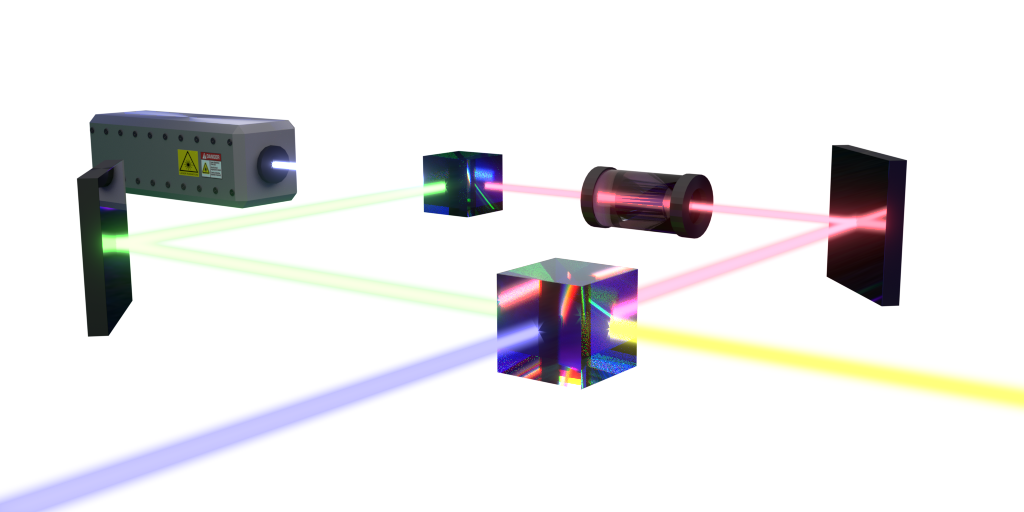
\includegraphics[width=0.8\hsize]{img/cover3Dpicture.png}
\vfill

% Bottom of the page
{\large \today}

\end{center}

\cleardoublepage
\cleardoublepage
\setcounter{page}{1}

%%%%%%%%%%%%%%%%%%%%%%%%
% DEDICATION PAGE
%%%%%%%%%%%%%%%%%%%%%%%%
\vspace*{100pt}
\begin{center}
\emph{To my parents and my family}
\end{center}

\cleardoublepage

%%%%%%%%%%%%%%%%%%%%%%%%
% HEADINGS AND PAGE NUM.
%%%%%%%%%%%%%%%%%%%%%%%%

\renewcommand{\rightmark}{\bf \thesubsection}
\renewcommand{\headrulewidth}{0.5pt}
\fancyfoot[LE,RO]{\thepage}
\fancyhead[LE]{Section: \rightmark} % TODO: Solve heading
\fancyhead[RO]{\leftmark}

%%%%%%%%%%%%%%%%%%%%%%%%
% REDEFINE TITLE FORMAT
%%%%%%%%%%%%%%%%%%%%%%%%
\titleformat{\section}[display]
{\vspace*{190pt}
\bf\Huge}
{\begin{picture}(0,0)\put(-64,-31){\textcolor{grey}{\thesection}}\end{picture}}
{0pt}
{\textcolor{withe}{#1}}
[]
\titlespacing*{\section}{100pt}{10pt}{40pt}[40pt]


\section{Introduction}
\thiswatermark{\put(1,-297){\color{l-grey}\rule{84pt}{42pt}}
\put(84,-297){\color{grey}\rule{410pt}{42pt}}}

%!TEX root = main.tex

% Section: Introduction
\lettrine[lines=2, findent=3pt,nindent=0pt]{M}{etrology} has played an inportant role since [TODO: add historical reasons]. With the development of quantum technology, a more deep understanding of one of its aspect as the quantum metrology is needed. Therefore, many works appeared recently on the literature. 

In this work the author, in collaboration with other researchers [TODO: see how to add reference to the rest of collavorators], has addressed some crucial questions regarding this field. 


\section{\foreignlanguage{nohyphenation}{Background on Estimation and Quantum Information Theories}}
\thiswatermark{\put(1,-330){\color{l-grey}\rule{84pt}{75pt}}
\put(84,-330){\color{grey}\rule{410pt}{75pt}}}

\lettrine[lines=2, findent=3pt,nindent=0pt]{T}{his} thesis is based on
many previous works developed since long time ago.
It is known that estimation processes are part of different
aspects of the human been behaviour.
From the estimation of the season on which one has 
to plant some vegetables to grow until the estimation of which route is the
shorter to reach somewhere. 
All these processes usually involve a huge amount of data. 
So it has been developed a strongly consolidated theory around that.

%!TEX root = main.tex

Looking back to all that has occurred to me since that eventful day, I am 
scarcely able to believe in the reality of my adventures. They were truly
so wonderful that even now I am bewildered when I think of them.

My uncle was a German, having married my mother's sister, an Englishwoman. 
Being very much attached to his fatherless nephew, he invited me to study 
under him in his home in the fatherland. This home was in a large town, and 
my uncle a professor of philosophy, chemistry, geology, mineralogy, and many 
other ologies.

One day, after passing some hours in the laboratory�my uncle being absent 
at the time�I suddenly felt the necessity of renovating the tissues�i.e., 
I was hungry, and was about to rouse up our old French cook, when my uncle, 
Professor Von Hardwigg, suddenly opened the street door, and came rushing 
upstairs.

Now Professor Hardwigg, my worthy uncle, is by no means a bad sort of man; 
he is, however, choleric and original. To bear with him means to obey; and 
scarcely had his heavy feet resounded within our joint domicile than he 
shouted for me to attend upon him.

'Harry�Harry�Harry�'

I hastened to obey, but before I could reach his room, jumping three steps 
at a time, he was stamping his right foot upon the landing.

'Harry!' he cried, in a frantic tone, 'are you coming up?'

Now to tell the truth, at that moment I was far more interested in the 
question as to what was to constitute our dinner than in any problem of 
science; to me soup was more interesting than soda, an omelette more 
tempting than arithmetic, and an artichoke of ten times more value than 
any amount of asbestos.

But my uncle was not a man to be kept waiting; so adjourning therefore 
all minor questions, I presented myself before him.

He was a very learned man. Now most persons in this category supply 
themselves with information, as peddlers do with goods, for the benefit 
of others, and lay up stores in order to diffuse them abroad for the 
benefit of society in general. Not so my excellent uncle, Professor 
Hardwigg; he studied, he consumed the midnight oil, he pored over heavy 
tomes, and digested huge quartos and folios in order to keep the knowledge 
acquired to himself.

There was a reason, and it may be regarded as a good one, why my uncle 
objected to display his learning more than was absolutely necessary: he 
stammered; and when intent upon explaining the phenomena of the heavens, 
was apt to find himself at fault, and allude in such a vague way to sun, 
moon, and stars that few were able to comprehend his meaning. To tell 
the honest truth, when the right word would not come, it was generally 
replaced by a very powerful adjective.

In connection with the sciences there are many almost unpronounceable 
names�names very much resembling those of Welsh villages; and my uncle 
being very fond of using them, his habit of stammering was not thereby 
improved. In fact, there were periods in his discourse when he would 
finally give up and swallow his discomfiture�in a glass of water.

As I said, my uncle, Professor Hardwigg, was a very learned man; and I 
now add a most kind relative. I was bound to him by the double ties of 
affection and interest. I took deep interest in all his doings, and 
hoped some day to be almost as learned myself. It was a rare thing for 
me to be absent from his lectures. Like him, I preferred mineralogy to 
all the other sciences. My anxiety was to gain real knowledge of the 
earth. Geology and mineralogy were to us the sole objects of life, and 
in connection with these studies many a fair specimen of stone, chalk, 
or metal did we break with our hammers.

Steel rods, loadstones, glass pipes, and bottles of various acids were 
oftener before us than our meals. My uncle Hardwigg was once known to 
classify six hundred different geological specimens by their weight, 
hardness, fusibility, sound, taste, and smell.

He corresponded with all the great, learned, and scientific men of the 
age. I was, therefore, in constant communication with, at all events the 
letters of, Sir Humphry Davy, Captain Franklin, and other great men.

But before I state the subject on which my uncle wished to confer with me, 
I must say a word about his personal appearance. Alas! my readers will 
see a very different portrait of him at a future time, after he has gone 
through the fearful adventures yet to be related.

My uncle was fifty years old; tall, thin, and wiry. Large spectacles hid, 
to a certain extent, his vast, round, and goggle eyes, while his nose was 
irreverently compared to a thin file. So much indeed did it resemble that 
useful article, that a compass was said in his presence to have made 
considerable N (Nasal) deviation.

The truth being told, however, the only article really attracted to my 
uncle's nose was tobacco.

Another peculiarity of his was, that he always stepped a yard at a time, 
clenched his fists as if he were going to hit you, and was, when in one 
of his peculiar humors, very far from a pleasant companion.

It is further necessary to observe that he lived in a very nice house, 
in that very nice street, the Konigstrasse at Hamburg. Though lying in 
the center of a town, it was perfectly rural in its aspect�half wood, 
half bricks, with old fashioned gables�one of the few old houses spared 
by the great fire of 1842.

When I say a nice house, I mean a handsome house�old, tottering, and not 
exactly comfortable to English notions: a house a little off the 
perpendicular and inclined to fall into the neighboring canal; exactly 
the house for a wandering artist to depict; all the more that you could 
scarcely see it for ivy and a magnificent old tree which grew over the door.

My uncle was rich; his house was his own property, while he had a 
considerable private income. To my notion the best part of his possessions 
was his god daughter, Gretchen. And the old cook, the young lady, the 
Professor and I were the sole inhabitants.

I loved mineralogy, I loved geology. To me there was nothing like 
pebbles�and if my uncle had been in a little less of a fury, we should 
have been the happiest of families. To prove the excellent Hardwigg's 
impatience, I solemnly declare that when the flowers in the drawing room 
pots began to grow, he rose every morning at four o'clock to make them 
grow quicker by pulling the leaves!

Having described my uncle, I will now give an account of our interview.

He received me in his study; a perfect museum, containing every natural 
curiosity that can well be imagined�minerals, however, predominating. 
Every one was familiar to me, having been catalogued by my own hand. My 
uncle, apparently oblivious of the fact that he had summoned me to his 
presence, was absorbed in a book. He was particularly fond of early 
editions, tall copies, and unique works.

'Wonderful!' he cried, tapping his forehead. 'Wonderful wonderful!'

It was one of those yellow leaved volumes now rarely found on stalls, 
and to me it appeared to possess but little value. My uncle, however, 
was in raptures.

He admired its binding, the clearness of its characters, the ease with 
which it opened in his hand, and repeated aloud, half a dozen times, 
that it was very, very old.

To my fancy he was making a great fuss about nothing, but it was not my 
province to say so. On the contrary, I professed considerable interest 
in the subject, and asked him what it was about.

'It is the Heims Kringla of Snorre Tarleson,'he said, 'the celebrated 
Icelandic author of the twelfth century�it is a true and correct account 
of the Norwegian princes who reigned in Iceland.'

My next question related to the language in which it was written. I 
hoped at all events it was translated into German. My uncle was indignant 
at the very thought, and declared he wouldn't give a penny for a 
translation. His delight was to have found the original work in the 
Icelandic tongue, which he declared to be one of the most magnificent 
and yet simple idioms in the world�while at the same time its grammatical 
combinations were the most varied known to students.

'About as easy as German?' was my insidious remark.

My uncle shrugged his shoulders.

'The letters at all events,' I said, 'are rather difficult of comprehension.'

'It is a Runic manuscript, the language of the original population of 
Iceland, invented by Odin himself,' cried my uncle, angry at my ignorance.

I was about to venture upon some misplaced joke on the subject, when a 
small scrap of parchment fell out of the leaves. Like a hungry man 
snatching at a morsel of bread the Professor seized it. It was about 
five inches by three and was scrawled over in the most extraordinary fashion.

The lines shown here are an exact facsimile of what was written on 
the venerable piece of parchment and have wonderful importance, as 
they induced my uncle to undertake the most wonderful series of 
adventures which ever fell to the lot of human beings. 

\subsection{Classical estimation theory}
%!TEX root = main.tex

Looking back to all that has occurred to me since that eventful day, I am 
scarcely able to believe in the reality of my adventures. They were truly
so wonderful that even now I am bewildered when I think of them.

My uncle was a German, having married my mother's sister, an Englishwoman. 
Being very much attached to his fatherless nephew, he invited me to study 
under him in his home in the fatherland. This home was in a large town, and 
my uncle a professor of philosophy, chemistry, geology, mineralogy, and many 
other ologies.

One day, after passing some hours in the laboratory�my uncle being absent 
at the time�I suddenly felt the necessity of renovating the tissues�i.e., 
I was hungry, and was about to rouse up our old French cook, when my uncle, 
Professor Von Hardwigg, suddenly opened the street door, and came rushing 
upstairs.

Now Professor Hardwigg, my worthy uncle, is by no means a bad sort of man; 
he is, however, choleric and original. To bear with him means to obey; and 
scarcely had his heavy feet resounded within our joint domicile than he 
shouted for me to attend upon him.

'Harry�Harry�Harry�'

I hastened to obey, but before I could reach his room, jumping three steps 
at a time, he was stamping his right foot upon the landing.

'Harry!' he cried, in a frantic tone, 'are you coming up?'

Now to tell the truth, at that moment I was far more interested in the 
question as to what was to constitute our dinner than in any problem of 
science; to me soup was more interesting than soda, an omelette more 
tempting than arithmetic, and an artichoke of ten times more value than 
any amount of asbestos.

But my uncle was not a man to be kept waiting; so adjourning therefore 
all minor questions, I presented myself before him.

He was a very learned man. Now most persons in this category supply 
themselves with information, as peddlers do with goods, for the benefit 
of others, and lay up stores in order to diffuse them abroad for the 
benefit of society in general. Not so my excellent uncle, Professor 
Hardwigg; he studied, he consumed the midnight oil, he pored over heavy 
tomes, and digested huge quartos and folios in order to keep the knowledge 
acquired to himself.

There was a reason, and it may be regarded as a good one, why my uncle 
objected to display his learning more than was absolutely necessary: he 
stammered; and when intent upon explaining the phenomena of the heavens, 
was apt to find himself at fault, and allude in such a vague way to sun, 
moon, and stars that few were able to comprehend his meaning. To tell 
the honest truth, when the right word would not come, it was generally 
replaced by a very powerful adjective.

In connection with the sciences there are many almost unpronounceable 
names�names very much resembling those of Welsh villages; and my uncle 
being very fond of using them, his habit of stammering was not thereby 
improved. In fact, there were periods in his discourse when he would 
finally give up and swallow his discomfiture�in a glass of water.

As I said, my uncle, Professor Hardwigg, was a very learned man; and I 
now add a most kind relative. I was bound to him by the double ties of 
affection and interest. I took deep interest in all his doings, and 
hoped some day to be almost as learned myself. It was a rare thing for 
me to be absent from his lectures. Like him, I preferred mineralogy to 
all the other sciences. My anxiety was to gain real knowledge of the 
earth. Geology and mineralogy were to us the sole objects of life, and 
in connection with these studies many a fair specimen of stone, chalk, 
or metal did we break with our hammers.

Steel rods, loadstones, glass pipes, and bottles of various acids were 
oftener before us than our meals. My uncle Hardwigg was once known to 
classify six hundred different geological specimens by their weight, 
hardness, fusibility, sound, taste, and smell.

He corresponded with all the great, learned, and scientific men of the 
age. I was, therefore, in constant communication with, at all events the 
letters of, Sir Humphry Davy, Captain Franklin, and other great men.

But before I state the subject on which my uncle wished to confer with me, 
I must say a word about his personal appearance. Alas! my readers will 
see a very different portrait of him at a future time, after he has gone 
through the fearful adventures yet to be related.

My uncle was fifty years old; tall, thin, and wiry. Large spectacles hid, 
to a certain extent, his vast, round, and goggle eyes, while his nose was 
irreverently compared to a thin file. So much indeed did it resemble that 
useful article, that a compass was said in his presence to have made 
considerable N (Nasal) deviation.

The truth being told, however, the only article really attracted to my 
uncle's nose was tobacco.

Another peculiarity of his was, that he always stepped a yard at a time, 
clenched his fists as if he were going to hit you, and was, when in one 
of his peculiar humors, very far from a pleasant companion.

It is further necessary to observe that he lived in a very nice house, 
in that very nice street, the Konigstrasse at Hamburg. Though lying in 
the center of a town, it was perfectly rural in its aspect�half wood, 
half bricks, with old fashioned gables�one of the few old houses spared 
by the great fire of 1842.

When I say a nice house, I mean a handsome house�old, tottering, and not 
exactly comfortable to English notions: a house a little off the 
perpendicular and inclined to fall into the neighboring canal; exactly 
the house for a wandering artist to depict; all the more that you could 
scarcely see it for ivy and a magnificent old tree which grew over the door.

My uncle was rich; his house was his own property, while he had a 
considerable private income. To my notion the best part of his possessions 
was his god daughter, Gretchen. And the old cook, the young lady, the 
Professor and I were the sole inhabitants.

I loved mineralogy, I loved geology. To me there was nothing like 
pebbles�and if my uncle had been in a little less of a fury, we should 
have been the happiest of families. To prove the excellent Hardwigg's 
impatience, I solemnly declare that when the flowers in the drawing room 
pots began to grow, he rose every morning at four o'clock to make them 
grow quicker by pulling the leaves!

Having described my uncle, I will now give an account of our interview.

He received me in his study; a perfect museum, containing every natural 
curiosity that can well be imagined�minerals, however, predominating. 
Every one was familiar to me, having been catalogued by my own hand. My 
uncle, apparently oblivious of the fact that he had summoned me to his 
presence, was absorbed in a book. He was particularly fond of early 
editions, tall copies, and unique works.

'Wonderful!' he cried, tapping his forehead. 'Wonderful wonderful!'

It was one of those yellow leaved volumes now rarely found on stalls, 
and to me it appeared to possess but little value. My uncle, however, 
was in raptures.

He admired its binding, the clearness of its characters, the ease with 
which it opened in his hand, and repeated aloud, half a dozen times, 
that it was very, very old.

To my fancy he was making a great fuss about nothing, but it was not my 
province to say so. On the contrary, I professed considerable interest 
in the subject, and asked him what it was about.

'It is the Heims Kringla of Snorre Tarleson,'he said, 'the celebrated 
Icelandic author of the twelfth century�it is a true and correct account 
of the Norwegian princes who reigned in Iceland.'

My next question related to the language in which it was written. I 
hoped at all events it was translated into German. My uncle was indignant 
at the very thought, and declared he wouldn't give a penny for a 
translation. His delight was to have found the original work in the 
Icelandic tongue, which he declared to be one of the most magnificent 
and yet simple idioms in the world�while at the same time its grammatical 
combinations were the most varied known to students.

'About as easy as German?' was my insidious remark.

My uncle shrugged his shoulders.

'The letters at all events,' I said, 'are rather difficult of comprehension.'

'It is a Runic manuscript, the language of the original population of 
Iceland, invented by Odin himself,' cried my uncle, angry at my ignorance.

I was about to venture upon some misplaced joke on the subject, when a 
small scrap of parchment fell out of the leaves. Like a hungry man 
snatching at a morsel of bread the Professor seized it. It was about 
five inches by three and was scrawled over in the most extraordinary fashion.

The lines shown here are an exact facsimile of what was written on 
the venerable piece of parchment and have wonderful importance, as 
they induced my uncle to undertake the most wonderful series of 
adventures which ever fell to the lot of human beings.

\subsection{Step in quantum estimation theory}
%!TEX root = main.tex

Looking back to all that has occurred to me since that eventful day, I am 
scarcely able to believe in the reality of my adventures. They were truly
so wonderful that even now I am bewildered when I think of them.

My uncle was a German, having married my mother's sister, an Englishwoman. 
Being very much attached to his fatherless nephew, he invited me to study 
under him in his home in the fatherland. This home was in a large town, and 
my uncle a professor of philosophy, chemistry, geology, mineralogy, and many 
other ologies.

One day, after passing some hours in the laboratory�my uncle being absent 
at the time�I suddenly felt the necessity of renovating the tissues�i.e., 
I was hungry, and was about to rouse up our old French cook, when my uncle, 
Professor Von Hardwigg, suddenly opened the street door, and came rushing 
upstairs.

Now Professor Hardwigg, my worthy uncle, is by no means a bad sort of man; 
he is, however, choleric and original. To bear with him means to obey; and 
scarcely had his heavy feet resounded within our joint domicile than he 
shouted for me to attend upon him.

'Harry�Harry�Harry�'

I hastened to obey, but before I could reach his room, jumping three steps 
at a time, he was stamping his right foot upon the landing.

'Harry!' he cried, in a frantic tone, 'are you coming up?'

Now to tell the truth, at that moment I was far more interested in the 
question as to what was to constitute our dinner than in any problem of 
science; to me soup was more interesting than soda, an omelette more 
tempting than arithmetic, and an artichoke of ten times more value than 
any amount of asbestos.

But my uncle was not a man to be kept waiting; so adjourning therefore 
all minor questions, I presented myself before him.

He was a very learned man. Now most persons in this category supply 
themselves with information, as peddlers do with goods, for the benefit 
of others, and lay up stores in order to diffuse them abroad for the 
benefit of society in general. Not so my excellent uncle, Professor 
Hardwigg; he studied, he consumed the midnight oil, he pored over heavy 
tomes, and digested huge quartos and folios in order to keep the knowledge 
acquired to himself.

There was a reason, and it may be regarded as a good one, why my uncle 
objected to display his learning more than was absolutely necessary: he 
stammered; and when intent upon explaining the phenomena of the heavens, 
was apt to find himself at fault, and allude in such a vague way to sun, 
moon, and stars that few were able to comprehend his meaning. To tell 
the honest truth, when the right word would not come, it was generally 
replaced by a very powerful adjective.

In connection with the sciences there are many almost unpronounceable 
names�names very much resembling those of Welsh villages; and my uncle 
being very fond of using them, his habit of stammering was not thereby 
improved. In fact, there were periods in his discourse when he would 
finally give up and swallow his discomfiture�in a glass of water.

As I said, my uncle, Professor Hardwigg, was a very learned man; and I 
now add a most kind relative. I was bound to him by the double ties of 
affection and interest. I took deep interest in all his doings, and 
hoped some day to be almost as learned myself. It was a rare thing for 
me to be absent from his lectures. Like him, I preferred mineralogy to 
all the other sciences. My anxiety was to gain real knowledge of the 
earth. Geology and mineralogy were to us the sole objects of life, and 
in connection with these studies many a fair specimen of stone, chalk, 
or metal did we break with our hammers.

Steel rods, loadstones, glass pipes, and bottles of various acids were 
oftener before us than our meals. My uncle Hardwigg was once known to 
classify six hundred different geological specimens by their weight, 
hardness, fusibility, sound, taste, and smell.

He corresponded with all the great, learned, and scientific men of the 
age. I was, therefore, in constant communication with, at all events the 
letters of, Sir Humphry Davy, Captain Franklin, and other great men.

But before I state the subject on which my uncle wished to confer with me, 
I must say a word about his personal appearance. Alas! my readers will 
see a very different portrait of him at a future time, after he has gone 
through the fearful adventures yet to be related.

My uncle was fifty years old; tall, thin, and wiry. Large spectacles hid, 
to a certain extent, his vast, round, and goggle eyes, while his nose was 
irreverently compared to a thin file. So much indeed did it resemble that 
useful article, that a compass was said in his presence to have made 
considerable N (Nasal) deviation.

The truth being told, however, the only article really attracted to my 
uncle's nose was tobacco.

Another peculiarity of his was, that he always stepped a yard at a time, 
clenched his fists as if he were going to hit you, and was, when in one 
of his peculiar humors, very far from a pleasant companion.

It is further necessary to observe that he lived in a very nice house, 
in that very nice street, the Konigstrasse at Hamburg. Though lying in 
the center of a town, it was perfectly rural in its aspect�half wood, 
half bricks, with old fashioned gables�one of the few old houses spared 
by the great fire of 1842.

When I say a nice house, I mean a handsome house�old, tottering, and not 
exactly comfortable to English notions: a house a little off the 
perpendicular and inclined to fall into the neighboring canal; exactly 
the house for a wandering artist to depict; all the more that you could 
scarcely see it for ivy and a magnificent old tree which grew over the door.

My uncle was rich; his house was his own property, while he had a 
considerable private income. To my notion the best part of his possessions 
was his god daughter, Gretchen. And the old cook, the young lady, the 
Professor and I were the sole inhabitants.

I loved mineralogy, I loved geology. To me there was nothing like 
pebbles�and if my uncle had been in a little less of a fury, we should 
have been the happiest of families. To prove the excellent Hardwigg's 
impatience, I solemnly declare that when the flowers in the drawing room 
pots began to grow, he rose every morning at four o'clock to make them 
grow quicker by pulling the leaves!

Having described my uncle, I will now give an account of our interview.

He received me in his study; a perfect museum, containing every natural 
curiosity that can well be imagined�minerals, however, predominating. 
Every one was familiar to me, having been catalogued by my own hand. My 
uncle, apparently oblivious of the fact that he had summoned me to his 
presence, was absorbed in a book. He was particularly fond of early 
editions, tall copies, and unique works.

'Wonderful!' he cried, tapping his forehead. 'Wonderful wonderful!'

It was one of those yellow leaved volumes now rarely found on stalls, 
and to me it appeared to possess but little value. My uncle, however, 
was in raptures.

He admired its binding, the clearness of its characters, the ease with 
which it opened in his hand, and repeated aloud, half a dozen times, 
that it was very, very old.

To my fancy he was making a great fuss about nothing, but it was not my 
province to say so. On the contrary, I professed considerable interest 
in the subject, and asked him what it was about.

'It is the Heims Kringla of Snorre Tarleson,'he said, 'the celebrated 
Icelandic author of the twelfth century�it is a true and correct account 
of the Norwegian princes who reigned in Iceland.'

My next question related to the language in which it was written. I 
hoped at all events it was translated into German. My uncle was indignant 
at the very thought, and declared he wouldn't give a penny for a 
translation. His delight was to have found the original work in the 
Icelandic tongue, which he declared to be one of the most magnificent 
and yet simple idioms in the world�while at the same time its grammatical 
combinations were the most varied known to students.

'About as easy as German?' was my insidious remark.

My uncle shrugged his shoulders.

'The letters at all events,' I said, 'are rather difficult of comprehension.'

'It is a Runic manuscript, the language of the original population of 
Iceland, invented by Odin himself,' cried my uncle, angry at my ignorance.

I was about to venture upon some misplaced joke on the subject, when a 
small scrap of parchment fell out of the leaves. Like a hungry man 
snatching at a morsel of bread the Professor seized it. It was about 
five inches by three and was scrawled over in the most extraordinary fashion.

The lines shown here are an exact facsimile of what was written on 
the venerable piece of parchment and have wonderful importance, as 
they induced my uncle to undertake the most wonderful series of 
adventures which ever fell to the lot of human beings.

\subsection{Quantum Metrology}
%!TEX root = main.tex

Looking back to all that has occurred to me since that eventful day, I am 
scarcely able to believe in the reality of my adventures. They were truly
so wonderful that even now I am bewildered when I think of them.

My uncle was a German, having married my mother's sister, an Englishwoman. 
Being very much attached to his fatherless nephew, he invited me to study 
under him in his home in the fatherland. This home was in a large town, and 
my uncle a professor of philosophy, chemistry, geology, mineralogy, and many 
other ologies.

One day, after passing some hours in the laboratory�my uncle being absent 
at the time�I suddenly felt the necessity of renovating the tissues�i.e., 
I was hungry, and was about to rouse up our old French cook, when my uncle, 
Professor Von Hardwigg, suddenly opened the street door, and came rushing 
upstairs.

Now Professor Hardwigg, my worthy uncle, is by no means a bad sort of man; 
he is, however, choleric and original. To bear with him means to obey; and 
scarcely had his heavy feet resounded within our joint domicile than he 
shouted for me to attend upon him.

'Harry�Harry�Harry�'

I hastened to obey, but before I could reach his room, jumping three steps 
at a time, he was stamping his right foot upon the landing.

'Harry!' he cried, in a frantic tone, 'are you coming up?'

Now to tell the truth, at that moment I was far more interested in the 
question as to what was to constitute our dinner than in any problem of 
science; to me soup was more interesting than soda, an omelette more 
tempting than arithmetic, and an artichoke of ten times more value than 
any amount of asbestos.

But my uncle was not a man to be kept waiting; so adjourning therefore 
all minor questions, I presented myself before him.

He was a very learned man. Now most persons in this category supply 
themselves with information, as peddlers do with goods, for the benefit 
of others, and lay up stores in order to diffuse them abroad for the 
benefit of society in general. Not so my excellent uncle, Professor 
Hardwigg; he studied, he consumed the midnight oil, he pored over heavy 
tomes, and digested huge quartos and folios in order to keep the knowledge 
acquired to himself.

There was a reason, and it may be regarded as a good one, why my uncle 
objected to display his learning more than was absolutely necessary: he 
stammered; and when intent upon explaining the phenomena of the heavens, 
was apt to find himself at fault, and allude in such a vague way to sun, 
moon, and stars that few were able to comprehend his meaning. To tell 
the honest truth, when the right word would not come, it was generally 
replaced by a very powerful adjective.

In connection with the sciences there are many almost unpronounceable 
names�names very much resembling those of Welsh villages; and my uncle 
being very fond of using them, his habit of stammering was not thereby 
improved. In fact, there were periods in his discourse when he would 
finally give up and swallow his discomfiture�in a glass of water.

As I said, my uncle, Professor Hardwigg, was a very learned man; and I 
now add a most kind relative. I was bound to him by the double ties of 
affection and interest. I took deep interest in all his doings, and 
hoped some day to be almost as learned myself. It was a rare thing for 
me to be absent from his lectures. Like him, I preferred mineralogy to 
all the other sciences. My anxiety was to gain real knowledge of the 
earth. Geology and mineralogy were to us the sole objects of life, and 
in connection with these studies many a fair specimen of stone, chalk, 
or metal did we break with our hammers.

Steel rods, loadstones, glass pipes, and bottles of various acids were 
oftener before us than our meals. My uncle Hardwigg was once known to 
classify six hundred different geological specimens by their weight, 
hardness, fusibility, sound, taste, and smell.

He corresponded with all the great, learned, and scientific men of the 
age. I was, therefore, in constant communication with, at all events the 
letters of, Sir Humphry Davy, Captain Franklin, and other great men.

But before I state the subject on which my uncle wished to confer with me, 
I must say a word about his personal appearance. Alas! my readers will 
see a very different portrait of him at a future time, after he has gone 
through the fearful adventures yet to be related.

My uncle was fifty years old; tall, thin, and wiry. Large spectacles hid, 
to a certain extent, his vast, round, and goggle eyes, while his nose was 
irreverently compared to a thin file. So much indeed did it resemble that 
useful article, that a compass was said in his presence to have made 
considerable N (Nasal) deviation.

The truth being told, however, the only article really attracted to my 
uncle's nose was tobacco.

Another peculiarity of his was, that he always stepped a yard at a time, 
clenched his fists as if he were going to hit you, and was, when in one 
of his peculiar humors, very far from a pleasant companion.

It is further necessary to observe that he lived in a very nice house, 
in that very nice street, the Konigstrasse at Hamburg. Though lying in 
the center of a town, it was perfectly rural in its aspect�half wood, 
half bricks, with old fashioned gables�one of the few old houses spared 
by the great fire of 1842.

When I say a nice house, I mean a handsome house�old, tottering, and not 
exactly comfortable to English notions: a house a little off the 
perpendicular and inclined to fall into the neighboring canal; exactly 
the house for a wandering artist to depict; all the more that you could 
scarcely see it for ivy and a magnificent old tree which grew over the door.

My uncle was rich; his house was his own property, while he had a 
considerable private income. To my notion the best part of his possessions 
was his god daughter, Gretchen. And the old cook, the young lady, the 
Professor and I were the sole inhabitants.

I loved mineralogy, I loved geology. To me there was nothing like 
pebbles�and if my uncle had been in a little less of a fury, we should 
have been the happiest of families. To prove the excellent Hardwigg's 
impatience, I solemnly declare that when the flowers in the drawing room 
pots began to grow, he rose every morning at four o'clock to make them 
grow quicker by pulling the leaves!

Having described my uncle, I will now give an account of our interview.

He received me in his study; a perfect museum, containing every natural 
curiosity that can well be imagined�minerals, however, predominating. 
Every one was familiar to me, having been catalogued by my own hand. My 
uncle, apparently oblivious of the fact that he had summoned me to his 
presence, was absorbed in a book. He was particularly fond of early 
editions, tall copies, and unique works.

'Wonderful!' he cried, tapping his forehead. 'Wonderful wonderful!'

It was one of those yellow leaved volumes now rarely found on stalls, 
and to me it appeared to possess but little value. My uncle, however, 
was in raptures.

He admired its binding, the clearness of its characters, the ease with 
which it opened in his hand, and repeated aloud, half a dozen times, 
that it was very, very old.

To my fancy he was making a great fuss about nothing, but it was not my 
province to say so. On the contrary, I professed considerable interest 
in the subject, and asked him what it was about.

'It is the Heims Kringla of Snorre Tarleson,'he said, 'the celebrated 
Icelandic author of the twelfth century�it is a true and correct account 
of the Norwegian princes who reigned in Iceland.'

My next question related to the language in which it was written. I 
hoped at all events it was translated into German. My uncle was indignant 
at the very thought, and declared he wouldn't give a penny for a 
translation. His delight was to have found the original work in the 
Icelandic tongue, which he declared to be one of the most magnificent 
and yet simple idioms in the world�while at the same time its grammatical 
combinations were the most varied known to students.

'About as easy as German?' was my insidious remark.

My uncle shrugged his shoulders.

'The letters at all events,' I said, 'are rather difficult of comprehension.'

'It is a Runic manuscript, the language of the original population of 
Iceland, invented by Odin himself,' cried my uncle, angry at my ignorance.

I was about to venture upon some misplaced joke on the subject, when a 
small scrap of parchment fell out of the leaves. Like a hungry man 
snatching at a morsel of bread the Professor seized it. It was about 
five inches by three and was scrawled over in the most extraordinary fashion.

The lines shown here are an exact facsimile of what was written on 
the venerable piece of parchment and have wonderful importance, as 
they induced my uncle to undertake the most wonderful series of 
adventures which ever fell to the lot of human beings.

\section{Quantum metrology with Dicke like states}
\thiswatermark{\put(1,-327){\color{l-grey}\rule{84pt}{72pt}}
\put(84,-327){\color{grey}\rule{410pt}{72pt}}} 
%!TEX root = main.tex

Looking back to all that has occurred to me since that eventful day, I am 
scarcely able to believe in the reality of my adventures. They were truly
so wonderful that even now I am bewildered when I think of them.

My uncle was a German, having married my mother's sister, an Englishwoman. 
Being very much attached to his fatherless nephew, he invited me to study 
under him in his home in the fatherland. This home was in a large town, and 
my uncle a professor of philosophy, chemistry, geology, mineralogy, and many 
other ologies.

One day, after passing some hours in the laboratory�my uncle being absent 
at the time�I suddenly felt the necessity of renovating the tissues�i.e., 
I was hungry, and was about to rouse up our old French cook, when my uncle, 
Professor Von Hardwigg, suddenly opened the street door, and came rushing 
upstairs.

Now Professor Hardwigg, my worthy uncle, is by no means a bad sort of man; 
he is, however, choleric and original. To bear with him means to obey; and 
scarcely had his heavy feet resounded within our joint domicile than he 
shouted for me to attend upon him.

'Harry�Harry�Harry�'

I hastened to obey, but before I could reach his room, jumping three steps 
at a time, he was stamping his right foot upon the landing.

'Harry!' he cried, in a frantic tone, 'are you coming up?'

Now to tell the truth, at that moment I was far more interested in the 
question as to what was to constitute our dinner than in any problem of 
science; to me soup was more interesting than soda, an omelette more 
tempting than arithmetic, and an artichoke of ten times more value than 
any amount of asbestos.

But my uncle was not a man to be kept waiting; so adjourning therefore 
all minor questions, I presented myself before him.

He was a very learned man. Now most persons in this category supply 
themselves with information, as peddlers do with goods, for the benefit 
of others, and lay up stores in order to diffuse them abroad for the 
benefit of society in general. Not so my excellent uncle, Professor 
Hardwigg; he studied, he consumed the midnight oil, he pored over heavy 
tomes, and digested huge quartos and folios in order to keep the knowledge 
acquired to himself.

There was a reason, and it may be regarded as a good one, why my uncle 
objected to display his learning more than was absolutely necessary: he 
stammered; and when intent upon explaining the phenomena of the heavens, 
was apt to find himself at fault, and allude in such a vague way to sun, 
moon, and stars that few were able to comprehend his meaning. To tell 
the honest truth, when the right word would not come, it was generally 
replaced by a very powerful adjective.

In connection with the sciences there are many almost unpronounceable 
names�names very much resembling those of Welsh villages; and my uncle 
being very fond of using them, his habit of stammering was not thereby 
improved. In fact, there were periods in his discourse when he would 
finally give up and swallow his discomfiture�in a glass of water.

As I said, my uncle, Professor Hardwigg, was a very learned man; and I 
now add a most kind relative. I was bound to him by the double ties of 
affection and interest. I took deep interest in all his doings, and 
hoped some day to be almost as learned myself. It was a rare thing for 
me to be absent from his lectures. Like him, I preferred mineralogy to 
all the other sciences. My anxiety was to gain real knowledge of the 
earth. Geology and mineralogy were to us the sole objects of life, and 
in connection with these studies many a fair specimen of stone, chalk, 
or metal did we break with our hammers.

Steel rods, loadstones, glass pipes, and bottles of various acids were 
oftener before us than our meals. My uncle Hardwigg was once known to 
classify six hundred different geological specimens by their weight, 
hardness, fusibility, sound, taste, and smell.

He corresponded with all the great, learned, and scientific men of the 
age. I was, therefore, in constant communication with, at all events the 
letters of, Sir Humphry Davy, Captain Franklin, and other great men.

But before I state the subject on which my uncle wished to confer with me, 
I must say a word about his personal appearance. Alas! my readers will 
see a very different portrait of him at a future time, after he has gone 
through the fearful adventures yet to be related.

My uncle was fifty years old; tall, thin, and wiry. Large spectacles hid, 
to a certain extent, his vast, round, and goggle eyes, while his nose was 
irreverently compared to a thin file. So much indeed did it resemble that 
useful article, that a compass was said in his presence to have made 
considerable N (Nasal) deviation.

The truth being told, however, the only article really attracted to my 
uncle's nose was tobacco.

Another peculiarity of his was, that he always stepped a yard at a time, 
clenched his fists as if he were going to hit you, and was, when in one 
of his peculiar humors, very far from a pleasant companion.

It is further necessary to observe that he lived in a very nice house, 
in that very nice street, the Konigstrasse at Hamburg. Though lying in 
the center of a town, it was perfectly rural in its aspect�half wood, 
half bricks, with old fashioned gables�one of the few old houses spared 
by the great fire of 1842.

When I say a nice house, I mean a handsome house�old, tottering, and not 
exactly comfortable to English notions: a house a little off the 
perpendicular and inclined to fall into the neighboring canal; exactly 
the house for a wandering artist to depict; all the more that you could 
scarcely see it for ivy and a magnificent old tree which grew over the door.

My uncle was rich; his house was his own property, while he had a 
considerable private income. To my notion the best part of his possessions 
was his god daughter, Gretchen. And the old cook, the young lady, the 
Professor and I were the sole inhabitants.

I loved mineralogy, I loved geology. To me there was nothing like 
pebbles�and if my uncle had been in a little less of a fury, we should 
have been the happiest of families. To prove the excellent Hardwigg's 
impatience, I solemnly declare that when the flowers in the drawing room 
pots began to grow, he rose every morning at four o'clock to make them 
grow quicker by pulling the leaves!

Having described my uncle, I will now give an account of our interview.

He received me in his study; a perfect museum, containing every natural 
curiosity that can well be imagined�minerals, however, predominating. 
Every one was familiar to me, having been catalogued by my own hand. My 
uncle, apparently oblivious of the fact that he had summoned me to his 
presence, was absorbed in a book. He was particularly fond of early 
editions, tall copies, and unique works.

'Wonderful!' he cried, tapping his forehead. 'Wonderful wonderful!'

It was one of those yellow leaved volumes now rarely found on stalls, 
and to me it appeared to possess but little value. My uncle, however, 
was in raptures.

He admired its binding, the clearness of its characters, the ease with 
which it opened in his hand, and repeated aloud, half a dozen times, 
that it was very, very old.

To my fancy he was making a great fuss about nothing, but it was not my 
province to say so. On the contrary, I professed considerable interest 
in the subject, and asked him what it was about.

'It is the Heims Kringla of Snorre Tarleson,'he said, 'the celebrated 
Icelandic author of the twelfth century�it is a true and correct account 
of the Norwegian princes who reigned in Iceland.'

My next question related to the language in which it was written. I 
hoped at all events it was translated into German. My uncle was indignant 
at the very thought, and declared he wouldn't give a penny for a 
translation. His delight was to have found the original work in the 
Icelandic tongue, which he declared to be one of the most magnificent 
and yet simple idioms in the world�while at the same time its grammatical 
combinations were the most varied known to students.

'About as easy as German?' was my insidious remark.

My uncle shrugged his shoulders.

'The letters at all events,' I said, 'are rather difficult of comprehension.'

'It is a Runic manuscript, the language of the original population of 
Iceland, invented by Odin himself,' cried my uncle, angry at my ignorance.

I was about to venture upon some misplaced joke on the subject, when a 
small scrap of parchment fell out of the leaves. Like a hungry man 
snatching at a morsel of bread the Professor seized it. It was about 
five inches by three and was scrawled over in the most extraordinary fashion.

The lines shown here are an exact facsimile of what was written on 
the venerable piece of parchment and have wonderful importance, as 
they induced my uncle to undertake the most wonderful series of 
adventures which ever fell to the lot of human beings.

\section[Bounding qFI with observables]
{Bounding quantum Fisher \qquad\qquad\, Information with observables}
\thiswatermark{\put(1,-327){\color{l-grey}\rule{84pt}{72pt}}
\put(84,-327){\color{grey}\rule{410pt}{72pt}}} 
%!TEX root = main.tex

Looking back to all that has occurred to me since that eventful day, I am 
scarcely able to believe in the reality of my adventures. They were truly
so wonderful that even now I am bewildered when I think of them.

My uncle was a German, having married my mother's sister, an Englishwoman. 
Being very much attached to his fatherless nephew, he invited me to study 
under him in his home in the fatherland. This home was in a large town, and 
my uncle a professor of philosophy, chemistry, geology, mineralogy, and many 
other ologies.

One day, after passing some hours in the laboratory�my uncle being absent 
at the time�I suddenly felt the necessity of renovating the tissues�i.e., 
I was hungry, and was about to rouse up our old French cook, when my uncle, 
Professor Von Hardwigg, suddenly opened the street door, and came rushing 
upstairs.

Now Professor Hardwigg, my worthy uncle, is by no means a bad sort of man; 
he is, however, choleric and original. To bear with him means to obey; and 
scarcely had his heavy feet resounded within our joint domicile than he 
shouted for me to attend upon him.

'Harry�Harry�Harry�'

I hastened to obey, but before I could reach his room, jumping three steps 
at a time, he was stamping his right foot upon the landing.

'Harry!' he cried, in a frantic tone, 'are you coming up?'

Now to tell the truth, at that moment I was far more interested in the 
question as to what was to constitute our dinner than in any problem of 
science; to me soup was more interesting than soda, an omelette more 
tempting than arithmetic, and an artichoke of ten times more value than 
any amount of asbestos.

But my uncle was not a man to be kept waiting; so adjourning therefore 
all minor questions, I presented myself before him.

He was a very learned man. Now most persons in this category supply 
themselves with information, as peddlers do with goods, for the benefit 
of others, and lay up stores in order to diffuse them abroad for the 
benefit of society in general. Not so my excellent uncle, Professor 
Hardwigg; he studied, he consumed the midnight oil, he pored over heavy 
tomes, and digested huge quartos and folios in order to keep the knowledge 
acquired to himself.

There was a reason, and it may be regarded as a good one, why my uncle 
objected to display his learning more than was absolutely necessary: he 
stammered; and when intent upon explaining the phenomena of the heavens, 
was apt to find himself at fault, and allude in such a vague way to sun, 
moon, and stars that few were able to comprehend his meaning. To tell 
the honest truth, when the right word would not come, it was generally 
replaced by a very powerful adjective.

In connection with the sciences there are many almost unpronounceable 
names�names very much resembling those of Welsh villages; and my uncle 
being very fond of using them, his habit of stammering was not thereby 
improved. In fact, there were periods in his discourse when he would 
finally give up and swallow his discomfiture�in a glass of water.

As I said, my uncle, Professor Hardwigg, was a very learned man; and I 
now add a most kind relative. I was bound to him by the double ties of 
affection and interest. I took deep interest in all his doings, and 
hoped some day to be almost as learned myself. It was a rare thing for 
me to be absent from his lectures. Like him, I preferred mineralogy to 
all the other sciences. My anxiety was to gain real knowledge of the 
earth. Geology and mineralogy were to us the sole objects of life, and 
in connection with these studies many a fair specimen of stone, chalk, 
or metal did we break with our hammers.

Steel rods, loadstones, glass pipes, and bottles of various acids were 
oftener before us than our meals. My uncle Hardwigg was once known to 
classify six hundred different geological specimens by their weight, 
hardness, fusibility, sound, taste, and smell.

He corresponded with all the great, learned, and scientific men of the 
age. I was, therefore, in constant communication with, at all events the 
letters of, Sir Humphry Davy, Captain Franklin, and other great men.

But before I state the subject on which my uncle wished to confer with me, 
I must say a word about his personal appearance. Alas! my readers will 
see a very different portrait of him at a future time, after he has gone 
through the fearful adventures yet to be related.

My uncle was fifty years old; tall, thin, and wiry. Large spectacles hid, 
to a certain extent, his vast, round, and goggle eyes, while his nose was 
irreverently compared to a thin file. So much indeed did it resemble that 
useful article, that a compass was said in his presence to have made 
considerable N (Nasal) deviation.

The truth being told, however, the only article really attracted to my 
uncle's nose was tobacco.

Another peculiarity of his was, that he always stepped a yard at a time, 
clenched his fists as if he were going to hit you, and was, when in one 
of his peculiar humors, very far from a pleasant companion.

It is further necessary to observe that he lived in a very nice house, 
in that very nice street, the Konigstrasse at Hamburg. Though lying in 
the center of a town, it was perfectly rural in its aspect�half wood, 
half bricks, with old fashioned gables�one of the few old houses spared 
by the great fire of 1842.

When I say a nice house, I mean a handsome house�old, tottering, and not 
exactly comfortable to English notions: a house a little off the 
perpendicular and inclined to fall into the neighboring canal; exactly 
the house for a wandering artist to depict; all the more that you could 
scarcely see it for ivy and a magnificent old tree which grew over the door.

My uncle was rich; his house was his own property, while he had a 
considerable private income. To my notion the best part of his possessions 
was his god daughter, Gretchen. And the old cook, the young lady, the 
Professor and I were the sole inhabitants.

I loved mineralogy, I loved geology. To me there was nothing like 
pebbles�and if my uncle had been in a little less of a fury, we should 
have been the happiest of families. To prove the excellent Hardwigg's 
impatience, I solemnly declare that when the flowers in the drawing room 
pots began to grow, he rose every morning at four o'clock to make them 
grow quicker by pulling the leaves!

Having described my uncle, I will now give an account of our interview.

He received me in his study; a perfect museum, containing every natural 
curiosity that can well be imagined�minerals, however, predominating. 
Every one was familiar to me, having been catalogued by my own hand. My 
uncle, apparently oblivious of the fact that he had summoned me to his 
presence, was absorbed in a book. He was particularly fond of early 
editions, tall copies, and unique works.

'Wonderful!' he cried, tapping his forehead. 'Wonderful wonderful!'

It was one of those yellow leaved volumes now rarely found on stalls, 
and to me it appeared to possess but little value. My uncle, however, 
was in raptures.

He admired its binding, the clearness of its characters, the ease with 
which it opened in his hand, and repeated aloud, half a dozen times, 
that it was very, very old.

To my fancy he was making a great fuss about nothing, but it was not my 
province to say so. On the contrary, I professed considerable interest 
in the subject, and asked him what it was about.

'It is the Heims Kringla of Snorre Tarleson,'he said, 'the celebrated 
Icelandic author of the twelfth century�it is a true and correct account 
of the Norwegian princes who reigned in Iceland.'

My next question related to the language in which it was written. I 
hoped at all events it was translated into German. My uncle was indignant 
at the very thought, and declared he wouldn't give a penny for a 
translation. His delight was to have found the original work in the 
Icelandic tongue, which he declared to be one of the most magnificent 
and yet simple idioms in the world�while at the same time its grammatical 
combinations were the most varied known to students.

'About as easy as German?' was my insidious remark.

My uncle shrugged his shoulders.

'The letters at all events,' I said, 'are rather difficult of comprehension.'

'It is a Runic manuscript, the language of the original population of 
Iceland, invented by Odin himself,' cried my uncle, angry at my ignorance.

I was about to venture upon some misplaced joke on the subject, when a 
small scrap of parchment fell out of the leaves. Like a hungry man 
snatching at a morsel of bread the Professor seized it. It was about 
five inches by three and was scrawled over in the most extraordinary fashion.

The lines shown here are an exact facsimile of what was written on 
the venerable piece of parchment and have wonderful importance, as 
they induced my uncle to undertake the most wonderful series of 
adventures which ever fell to the lot of human beings.

\section{Accuracy bound for gradient field estimation with atomic ensembles}
\thiswatermark{\put(1,-327){\color{l-grey}\rule{84pt}{72pt}}
\put(84,-327){\color{grey}\rule{410pt}{72pt}}} 
%!TEX root = main.tex

Looking back to all that has occurred to me since that eventful day, I am 
scarcely able to believe in the reality of my adventures. They were truly
so wonderful that even now I am bewildered when I think of them.

My uncle was a German, having married my mother's sister, an Englishwoman. 
Being very much attached to his fatherless nephew, he invited me to study 
under him in his home in the fatherland. This home was in a large town, and 
my uncle a professor of philosophy, chemistry, geology, mineralogy, and many 
other ologies.

One day, after passing some hours in the laboratory�my uncle being absent 
at the time�I suddenly felt the necessity of renovating the tissues�i.e., 
I was hungry, and was about to rouse up our old French cook, when my uncle, 
Professor Von Hardwigg, suddenly opened the street door, and came rushing 
upstairs.

Now Professor Hardwigg, my worthy uncle, is by no means a bad sort of man; 
he is, however, choleric and original. To bear with him means to obey; and 
scarcely had his heavy feet resounded within our joint domicile than he 
shouted for me to attend upon him.

'Harry�Harry�Harry�'

I hastened to obey, but before I could reach his room, jumping three steps 
at a time, he was stamping his right foot upon the landing.

'Harry!' he cried, in a frantic tone, 'are you coming up?'

Now to tell the truth, at that moment I was far more interested in the 
question as to what was to constitute our dinner than in any problem of 
science; to me soup was more interesting than soda, an omelette more 
tempting than arithmetic, and an artichoke of ten times more value than 
any amount of asbestos.

But my uncle was not a man to be kept waiting; so adjourning therefore 
all minor questions, I presented myself before him.

He was a very learned man. Now most persons in this category supply 
themselves with information, as peddlers do with goods, for the benefit 
of others, and lay up stores in order to diffuse them abroad for the 
benefit of society in general. Not so my excellent uncle, Professor 
Hardwigg; he studied, he consumed the midnight oil, he pored over heavy 
tomes, and digested huge quartos and folios in order to keep the knowledge 
acquired to himself.

There was a reason, and it may be regarded as a good one, why my uncle 
objected to display his learning more than was absolutely necessary: he 
stammered; and when intent upon explaining the phenomena of the heavens, 
was apt to find himself at fault, and allude in such a vague way to sun, 
moon, and stars that few were able to comprehend his meaning. To tell 
the honest truth, when the right word would not come, it was generally 
replaced by a very powerful adjective.

In connection with the sciences there are many almost unpronounceable 
names�names very much resembling those of Welsh villages; and my uncle 
being very fond of using them, his habit of stammering was not thereby 
improved. In fact, there were periods in his discourse when he would 
finally give up and swallow his discomfiture�in a glass of water.

As I said, my uncle, Professor Hardwigg, was a very learned man; and I 
now add a most kind relative. I was bound to him by the double ties of 
affection and interest. I took deep interest in all his doings, and 
hoped some day to be almost as learned myself. It was a rare thing for 
me to be absent from his lectures. Like him, I preferred mineralogy to 
all the other sciences. My anxiety was to gain real knowledge of the 
earth. Geology and mineralogy were to us the sole objects of life, and 
in connection with these studies many a fair specimen of stone, chalk, 
or metal did we break with our hammers.

Steel rods, loadstones, glass pipes, and bottles of various acids were 
oftener before us than our meals. My uncle Hardwigg was once known to 
classify six hundred different geological specimens by their weight, 
hardness, fusibility, sound, taste, and smell.

He corresponded with all the great, learned, and scientific men of the 
age. I was, therefore, in constant communication with, at all events the 
letters of, Sir Humphry Davy, Captain Franklin, and other great men.

But before I state the subject on which my uncle wished to confer with me, 
I must say a word about his personal appearance. Alas! my readers will 
see a very different portrait of him at a future time, after he has gone 
through the fearful adventures yet to be related.

My uncle was fifty years old; tall, thin, and wiry. Large spectacles hid, 
to a certain extent, his vast, round, and goggle eyes, while his nose was 
irreverently compared to a thin file. So much indeed did it resemble that 
useful article, that a compass was said in his presence to have made 
considerable N (Nasal) deviation.

The truth being told, however, the only article really attracted to my 
uncle's nose was tobacco.

Another peculiarity of his was, that he always stepped a yard at a time, 
clenched his fists as if he were going to hit you, and was, when in one 
of his peculiar humors, very far from a pleasant companion.

It is further necessary to observe that he lived in a very nice house, 
in that very nice street, the Konigstrasse at Hamburg. Though lying in 
the center of a town, it was perfectly rural in its aspect�half wood, 
half bricks, with old fashioned gables�one of the few old houses spared 
by the great fire of 1842.

When I say a nice house, I mean a handsome house�old, tottering, and not 
exactly comfortable to English notions: a house a little off the 
perpendicular and inclined to fall into the neighboring canal; exactly 
the house for a wandering artist to depict; all the more that you could 
scarcely see it for ivy and a magnificent old tree which grew over the door.

My uncle was rich; his house was his own property, while he had a 
considerable private income. To my notion the best part of his possessions 
was his god daughter, Gretchen. And the old cook, the young lady, the 
Professor and I were the sole inhabitants.

I loved mineralogy, I loved geology. To me there was nothing like 
pebbles�and if my uncle had been in a little less of a fury, we should 
have been the happiest of families. To prove the excellent Hardwigg's 
impatience, I solemnly declare that when the flowers in the drawing room 
pots began to grow, he rose every morning at four o'clock to make them 
grow quicker by pulling the leaves!

Having described my uncle, I will now give an account of our interview.

He received me in his study; a perfect museum, containing every natural 
curiosity that can well be imagined�minerals, however, predominating. 
Every one was familiar to me, having been catalogued by my own hand. My 
uncle, apparently oblivious of the fact that he had summoned me to his 
presence, was absorbed in a book. He was particularly fond of early 
editions, tall copies, and unique works.

'Wonderful!' he cried, tapping his forehead. 'Wonderful wonderful!'

It was one of those yellow leaved volumes now rarely found on stalls, 
and to me it appeared to possess but little value. My uncle, however, 
was in raptures.

He admired its binding, the clearness of its characters, the ease with 
which it opened in his hand, and repeated aloud, half a dozen times, 
that it was very, very old.

To my fancy he was making a great fuss about nothing, but it was not my 
province to say so. On the contrary, I professed considerable interest 
in the subject, and asked him what it was about.

'It is the Heims Kringla of Snorre Tarleson,'he said, 'the celebrated 
Icelandic author of the twelfth century�it is a true and correct account 
of the Norwegian princes who reigned in Iceland.'

My next question related to the language in which it was written. I 
hoped at all events it was translated into German. My uncle was indignant 
at the very thought, and declared he wouldn't give a penny for a 
translation. His delight was to have found the original work in the 
Icelandic tongue, which he declared to be one of the most magnificent 
and yet simple idioms in the world�while at the same time its grammatical 
combinations were the most varied known to students.

'About as easy as German?' was my insidious remark.

My uncle shrugged his shoulders.

'The letters at all events,' I said, 'are rather difficult of comprehension.'

'It is a Runic manuscript, the language of the original population of 
Iceland, invented by Odin himself,' cried my uncle, angry at my ignorance.

I was about to venture upon some misplaced joke on the subject, when a 
small scrap of parchment fell out of the leaves. Like a hungry man 
snatching at a morsel of bread the Professor seized it. It was about 
five inches by three and was scrawled over in the most extraordinary fashion.

The lines shown here are an exact facsimile of what was written on 
the venerable piece of parchment and have wonderful importance, as 
they induced my uncle to undertake the most wonderful series of 
adventures which ever fell to the lot of human beings.

%%%%%%%%%%%%%%%%%%%%%%%%
% REDEFINE TITLE FORMAT
%%%%%%%%%%%%%%%%%%%%%%%%
\titleformat{\section}[display]
{\vspace*{150pt}
\bf\Huge}
{\begin{picture}(0,0)\put(-60,-30){\textcolor{grey}{\thesection}}\end{picture}}
{0pt}
{#1}
[]
\titlespacing*{\section}{40pt}{10pt}{40pt}[40pt]

\section*{References}
%!TEX root = main.tex

Looking back to all that has occurred to me since that eventful day, I am 
scarcely able to believe in the reality of my adventures. They were truly
so wonderful that even now I am bewildered when I think of them.

My uncle was a German, having married my mother's sister, an Englishwoman. 
Being very much attached to his fatherless nephew, he invited me to study 
under him in his home in the fatherland. This home was in a large town, and 
my uncle a professor of philosophy, chemistry, geology, mineralogy, and many 
other ologies.

One day, after passing some hours in the laboratory�my uncle being absent 
at the time�I suddenly felt the necessity of renovating the tissues�i.e., 
I was hungry, and was about to rouse up our old French cook, when my uncle, 
Professor Von Hardwigg, suddenly opened the street door, and came rushing 
upstairs.

Now Professor Hardwigg, my worthy uncle, is by no means a bad sort of man; 
he is, however, choleric and original. To bear with him means to obey; and 
scarcely had his heavy feet resounded within our joint domicile than he 
shouted for me to attend upon him.

'Harry�Harry�Harry�'

I hastened to obey, but before I could reach his room, jumping three steps 
at a time, he was stamping his right foot upon the landing.

'Harry!' he cried, in a frantic tone, 'are you coming up?'

Now to tell the truth, at that moment I was far more interested in the 
question as to what was to constitute our dinner than in any problem of 
science; to me soup was more interesting than soda, an omelette more 
tempting than arithmetic, and an artichoke of ten times more value than 
any amount of asbestos.

But my uncle was not a man to be kept waiting; so adjourning therefore 
all minor questions, I presented myself before him.

He was a very learned man. Now most persons in this category supply 
themselves with information, as peddlers do with goods, for the benefit 
of others, and lay up stores in order to diffuse them abroad for the 
benefit of society in general. Not so my excellent uncle, Professor 
Hardwigg; he studied, he consumed the midnight oil, he pored over heavy 
tomes, and digested huge quartos and folios in order to keep the knowledge 
acquired to himself.

There was a reason, and it may be regarded as a good one, why my uncle 
objected to display his learning more than was absolutely necessary: he 
stammered; and when intent upon explaining the phenomena of the heavens, 
was apt to find himself at fault, and allude in such a vague way to sun, 
moon, and stars that few were able to comprehend his meaning. To tell 
the honest truth, when the right word would not come, it was generally 
replaced by a very powerful adjective.

In connection with the sciences there are many almost unpronounceable 
names�names very much resembling those of Welsh villages; and my uncle 
being very fond of using them, his habit of stammering was not thereby 
improved. In fact, there were periods in his discourse when he would 
finally give up and swallow his discomfiture�in a glass of water.

As I said, my uncle, Professor Hardwigg, was a very learned man; and I 
now add a most kind relative. I was bound to him by the double ties of 
affection and interest. I took deep interest in all his doings, and 
hoped some day to be almost as learned myself. It was a rare thing for 
me to be absent from his lectures. Like him, I preferred mineralogy to 
all the other sciences. My anxiety was to gain real knowledge of the 
earth. Geology and mineralogy were to us the sole objects of life, and 
in connection with these studies many a fair specimen of stone, chalk, 
or metal did we break with our hammers.

Steel rods, loadstones, glass pipes, and bottles of various acids were 
oftener before us than our meals. My uncle Hardwigg was once known to 
classify six hundred different geological specimens by their weight, 
hardness, fusibility, sound, taste, and smell.

He corresponded with all the great, learned, and scientific men of the 
age. I was, therefore, in constant communication with, at all events the 
letters of, Sir Humphry Davy, Captain Franklin, and other great men.

But before I state the subject on which my uncle wished to confer with me, 
I must say a word about his personal appearance. Alas! my readers will 
see a very different portrait of him at a future time, after he has gone 
through the fearful adventures yet to be related.

My uncle was fifty years old; tall, thin, and wiry. Large spectacles hid, 
to a certain extent, his vast, round, and goggle eyes, while his nose was 
irreverently compared to a thin file. So much indeed did it resemble that 
useful article, that a compass was said in his presence to have made 
considerable N (Nasal) deviation.

The truth being told, however, the only article really attracted to my 
uncle's nose was tobacco.

Another peculiarity of his was, that he always stepped a yard at a time, 
clenched his fists as if he were going to hit you, and was, when in one 
of his peculiar humors, very far from a pleasant companion.

It is further necessary to observe that he lived in a very nice house, 
in that very nice street, the Konigstrasse at Hamburg. Though lying in 
the center of a town, it was perfectly rural in its aspect�half wood, 
half bricks, with old fashioned gables�one of the few old houses spared 
by the great fire of 1842.

When I say a nice house, I mean a handsome house�old, tottering, and not 
exactly comfortable to English notions: a house a little off the 
perpendicular and inclined to fall into the neighboring canal; exactly 
the house for a wandering artist to depict; all the more that you could 
scarcely see it for ivy and a magnificent old tree which grew over the door.

My uncle was rich; his house was his own property, while he had a 
considerable private income. To my notion the best part of his possessions 
was his god daughter, Gretchen. And the old cook, the young lady, the 
Professor and I were the sole inhabitants.

I loved mineralogy, I loved geology. To me there was nothing like 
pebbles�and if my uncle had been in a little less of a fury, we should 
have been the happiest of families. To prove the excellent Hardwigg's 
impatience, I solemnly declare that when the flowers in the drawing room 
pots began to grow, he rose every morning at four o'clock to make them 
grow quicker by pulling the leaves!

Having described my uncle, I will now give an account of our interview.

He received me in his study; a perfect museum, containing every natural 
curiosity that can well be imagined�minerals, however, predominating. 
Every one was familiar to me, having been catalogued by my own hand. My 
uncle, apparently oblivious of the fact that he had summoned me to his 
presence, was absorbed in a book. He was particularly fond of early 
editions, tall copies, and unique works.

'Wonderful!' he cried, tapping his forehead. 'Wonderful wonderful!'

It was one of those yellow leaved volumes now rarely found on stalls, 
and to me it appeared to possess but little value. My uncle, however, 
was in raptures.

He admired its binding, the clearness of its characters, the ease with 
which it opened in his hand, and repeated aloud, half a dozen times, 
that it was very, very old.

To my fancy he was making a great fuss about nothing, but it was not my 
province to say so. On the contrary, I professed considerable interest 
in the subject, and asked him what it was about.

'It is the Heims Kringla of Snorre Tarleson,'he said, 'the celebrated 
Icelandic author of the twelfth century�it is a true and correct account 
of the Norwegian princes who reigned in Iceland.'

My next question related to the language in which it was written. I 
hoped at all events it was translated into German. My uncle was indignant 
at the very thought, and declared he wouldn't give a penny for a 
translation. His delight was to have found the original work in the 
Icelandic tongue, which he declared to be one of the most magnificent 
and yet simple idioms in the world�while at the same time its grammatical 
combinations were the most varied known to students.

'About as easy as German?' was my insidious remark.

My uncle shrugged his shoulders.

'The letters at all events,' I said, 'are rather difficult of comprehension.'

'It is a Runic manuscript, the language of the original population of 
Iceland, invented by Odin himself,' cried my uncle, angry at my ignorance.

I was about to venture upon some misplaced joke on the subject, when a 
small scrap of parchment fell out of the leaves. Like a hungry man 
snatching at a morsel of bread the Professor seized it. It was about 
five inches by three and was scrawled over in the most extraordinary fashion.

The lines shown here are an exact facsimile of what was written on 
the venerable piece of parchment and have wonderful importance, as 
they induced my uncle to undertake the most wonderful series of 
adventures which ever fell to the lot of human beings.

\section*{Index}
%!TEX root = main.tex

Looking back to all that has occurred to me since that eventful day, I am 
scarcely able to believe in the reality of my adventures. They were truly
so wonderful that even now I am bewildered when I think of them.

My uncle was a German, having married my mother's sister, an Englishwoman. 
Being very much attached to his fatherless nephew, he invited me to study 
under him in his home in the fatherland. This home was in a large town, and 
my uncle a professor of philosophy, chemistry, geology, mineralogy, and many 
other ologies.

One day, after passing some hours in the laboratory�my uncle being absent 
at the time�I suddenly felt the necessity of renovating the tissues�i.e., 
I was hungry, and was about to rouse up our old French cook, when my uncle, 
Professor Von Hardwigg, suddenly opened the street door, and came rushing 
upstairs.

Now Professor Hardwigg, my worthy uncle, is by no means a bad sort of man; 
he is, however, choleric and original. To bear with him means to obey; and 
scarcely had his heavy feet resounded within our joint domicile than he 
shouted for me to attend upon him.

'Harry�Harry�Harry�'

I hastened to obey, but before I could reach his room, jumping three steps 
at a time, he was stamping his right foot upon the landing.

'Harry!' he cried, in a frantic tone, 'are you coming up?'

Now to tell the truth, at that moment I was far more interested in the 
question as to what was to constitute our dinner than in any problem of 
science; to me soup was more interesting than soda, an omelette more 
tempting than arithmetic, and an artichoke of ten times more value than 
any amount of asbestos.

But my uncle was not a man to be kept waiting; so adjourning therefore 
all minor questions, I presented myself before him.

He was a very learned man. Now most persons in this category supply 
themselves with information, as peddlers do with goods, for the benefit 
of others, and lay up stores in order to diffuse them abroad for the 
benefit of society in general. Not so my excellent uncle, Professor 
Hardwigg; he studied, he consumed the midnight oil, he pored over heavy 
tomes, and digested huge quartos and folios in order to keep the knowledge 
acquired to himself.

There was a reason, and it may be regarded as a good one, why my uncle 
objected to display his learning more than was absolutely necessary: he 
stammered; and when intent upon explaining the phenomena of the heavens, 
was apt to find himself at fault, and allude in such a vague way to sun, 
moon, and stars that few were able to comprehend his meaning. To tell 
the honest truth, when the right word would not come, it was generally 
replaced by a very powerful adjective.

In connection with the sciences there are many almost unpronounceable 
names�names very much resembling those of Welsh villages; and my uncle 
being very fond of using them, his habit of stammering was not thereby 
improved. In fact, there were periods in his discourse when he would 
finally give up and swallow his discomfiture�in a glass of water.

As I said, my uncle, Professor Hardwigg, was a very learned man; and I 
now add a most kind relative. I was bound to him by the double ties of 
affection and interest. I took deep interest in all his doings, and 
hoped some day to be almost as learned myself. It was a rare thing for 
me to be absent from his lectures. Like him, I preferred mineralogy to 
all the other sciences. My anxiety was to gain real knowledge of the 
earth. Geology and mineralogy were to us the sole objects of life, and 
in connection with these studies many a fair specimen of stone, chalk, 
or metal did we break with our hammers.

Steel rods, loadstones, glass pipes, and bottles of various acids were 
oftener before us than our meals. My uncle Hardwigg was once known to 
classify six hundred different geological specimens by their weight, 
hardness, fusibility, sound, taste, and smell.

He corresponded with all the great, learned, and scientific men of the 
age. I was, therefore, in constant communication with, at all events the 
letters of, Sir Humphry Davy, Captain Franklin, and other great men.

But before I state the subject on which my uncle wished to confer with me, 
I must say a word about his personal appearance. Alas! my readers will 
see a very different portrait of him at a future time, after he has gone 
through the fearful adventures yet to be related.

My uncle was fifty years old; tall, thin, and wiry. Large spectacles hid, 
to a certain extent, his vast, round, and goggle eyes, while his nose was 
irreverently compared to a thin file. So much indeed did it resemble that 
useful article, that a compass was said in his presence to have made 
considerable N (Nasal) deviation.

The truth being told, however, the only article really attracted to my 
uncle's nose was tobacco.

Another peculiarity of his was, that he always stepped a yard at a time, 
clenched his fists as if he were going to hit you, and was, when in one 
of his peculiar humors, very far from a pleasant companion.

It is further necessary to observe that he lived in a very nice house, 
in that very nice street, the Konigstrasse at Hamburg. Though lying in 
the center of a town, it was perfectly rural in its aspect�half wood, 
half bricks, with old fashioned gables�one of the few old houses spared 
by the great fire of 1842.

When I say a nice house, I mean a handsome house�old, tottering, and not 
exactly comfortable to English notions: a house a little off the 
perpendicular and inclined to fall into the neighboring canal; exactly 
the house for a wandering artist to depict; all the more that you could 
scarcely see it for ivy and a magnificent old tree which grew over the door.

My uncle was rich; his house was his own property, while he had a 
considerable private income. To my notion the best part of his possessions 
was his god daughter, Gretchen. And the old cook, the young lady, the 
Professor and I were the sole inhabitants.

I loved mineralogy, I loved geology. To me there was nothing like 
pebbles�and if my uncle had been in a little less of a fury, we should 
have been the happiest of families. To prove the excellent Hardwigg's 
impatience, I solemnly declare that when the flowers in the drawing room 
pots began to grow, he rose every morning at four o'clock to make them 
grow quicker by pulling the leaves!

Having described my uncle, I will now give an account of our interview.

He received me in his study; a perfect museum, containing every natural 
curiosity that can well be imagined�minerals, however, predominating. 
Every one was familiar to me, having been catalogued by my own hand. My 
uncle, apparently oblivious of the fact that he had summoned me to his 
presence, was absorbed in a book. He was particularly fond of early 
editions, tall copies, and unique works.

'Wonderful!' he cried, tapping his forehead. 'Wonderful wonderful!'

It was one of those yellow leaved volumes now rarely found on stalls, 
and to me it appeared to possess but little value. My uncle, however, 
was in raptures.

He admired its binding, the clearness of its characters, the ease with 
which it opened in his hand, and repeated aloud, half a dozen times, 
that it was very, very old.

To my fancy he was making a great fuss about nothing, but it was not my 
province to say so. On the contrary, I professed considerable interest 
in the subject, and asked him what it was about.

'It is the Heims Kringla of Snorre Tarleson,'he said, 'the celebrated 
Icelandic author of the twelfth century�it is a true and correct account 
of the Norwegian princes who reigned in Iceland.'

My next question related to the language in which it was written. I 
hoped at all events it was translated into German. My uncle was indignant 
at the very thought, and declared he wouldn't give a penny for a 
translation. His delight was to have found the original work in the 
Icelandic tongue, which he declared to be one of the most magnificent 
and yet simple idioms in the world�while at the same time its grammatical 
combinations were the most varied known to students.

'About as easy as German?' was my insidious remark.

My uncle shrugged his shoulders.

'The letters at all events,' I said, 'are rather difficult of comprehension.'

'It is a Runic manuscript, the language of the original population of 
Iceland, invented by Odin himself,' cried my uncle, angry at my ignorance.

I was about to venture upon some misplaced joke on the subject, when a 
small scrap of parchment fell out of the leaves. Like a hungry man 
snatching at a morsel of bread the Professor seized it. It was about 
five inches by three and was scrawled over in the most extraordinary fashion.

The lines shown here are an exact facsimile of what was written on 
the venerable piece of parchment and have wonderful importance, as 
they induced my uncle to undertake the most wonderful series of 
adventures which ever fell to the lot of human beings.

\end{document}
